% Exact standardisation of 100 independent fair dice.
% Mean 350, variance 100*(35/12)=875/3, sigma=sqrt(875/3).
% Threshold 400 therefore z=50/sqrt(875/3)=sqrt(60/7).
\begin{tikzpicture}[x=1.15cm,y=1cm,line cap=round,>=stealth]
  \draw[->,black!65,thick] (-3.95,0)--(4.15,0);
  \foreach \z in {-3,-2,-1,0,1,2,3}{
    \draw[black!45] (\z,0.10)--(\z,-0.10);
    \node[below,font=\footnotesize] at (\z,-0.13) {$\z$};
  }
  \node[below,font=\footnotesize,anchor=west] at (3.56,-0.13) {$z$};
  \draw[MidnightBlue,very thick] (0,0)--(0,0.85);
  \node[above,font=\footnotesize,text=MidnightBlue,align=center] at (0,0.85) {mean $350$};
  \draw[BrickRed,very thick] (2.92770,0)--(2.92770,0.85);
  \node[above,font=\footnotesize,text=BrickRed,align=center] at (2.92770,0.85) {threshold $400$};
  \draw[<->,BrickRed!75,thick] (0,0.46)--(2.92770,0.46);
  \node[above,font=\footnotesize,fill=white,inner sep=1pt] at (1.48,0.47) {$50$ above mean};
  \node[font=\footnotesize,anchor=west] at (-3.65,-0.88)
    {$z=\dfrac{400-350}{\sqrt{100\cdot35/12}}=\sqrt{\dfrac{60}{7}}\approx2.93$};
\end{tikzpicture}
